%%%%%%%%%%%%%%%%%%%%%%%%%%%%%%%%%%%%%%%%%
% Beamer Presentation
% LaTeX Template
% Version 1.0 (10/11/12)
%
% This template has been downloaded from:
% http://www.LaTeXTemplates.com
%
% License:
% CC BY-NC-SA 3.0 (http://creativecommons.org/licenses/by-nc-sa/3.0/)
%
%%%%%%%%%%%%%%%%%%%%%%%%%%%%%%%%%%%%%%%%%

%----------------------------------------------------------------------------------------
%	PACKAGES AND THEMES
%----------------------------------------------------------------------------------------

\documentclass{beamer}

\mode<presentation> {

% The Beamer class comes with a number of default slide themes
% which change the colors and layouts of slides. Below this is a list
% of all the themes, uncomment each in turn to see what they look like.

%\usetheme{default}
%\usetheme{AnnArbor}
%\usetheme{Antibes}
%\usetheme{Bergen}
%\usetheme{Berkeley}
%\usetheme{Berlin}
%\usetheme{Boadilla}
%\usetheme{CambridgeUS}
%\usetheme{Copenhagen}
%\usetheme{Darmstadt}
%\usetheme{Dresden}
%\usetheme{Frankfurt}
%\usetheme{Goettingen}
%\usetheme{Hannover}
%\usetheme{Ilmenau}
%\usetheme{JuanLesPins}
%\usetheme{Luebeck}
\usetheme{Madrid}
%\usetheme{Malmoe}
%\usetheme{Marburg}
%\usetheme{Montpellier}
%\usetheme{PaloAlto}
%\usetheme{Pittsburgh}
%\usetheme{Rochester}
%\usetheme{Singapore}
%\usetheme{Szeged}
%\usetheme{Warsaw}

% As well as themes, the Beamer class has a number of color themes
% for any slide theme. Uncomment each of these in turn to see how it
% changes the colors of your current slide theme.

%\usecolortheme{albatross}
%\usecolortheme{beaver}
%\usecolortheme{beetle}
%\usecolortheme{crane}
%\usecolortheme{dolphin}
%\usecolortheme{dove}
%\usecolortheme{fly}
%\usecolortheme{lily}
%\usecolortheme{orchid}
%\usecolortheme{rose}
%\usecolortheme{seagull}
%\usecolortheme{seahorse}
%\usecolortheme{whale}
%\usecolortheme{wolverine}

%\setbeamertemplate{footline} % To remove the footer line in all slides uncomment this line
%\setbeamertemplate{footline}[page number] % To replace the footer line in all slides with a simple slide count uncomment this line

%\setbeamertemplate{navigation symbols}{} % To remove the navigation symbols from the bottom of all slides uncomment this line
}

\usepackage{graphicx} % Allows including images
\usepackage{booktabs} % Allows the use of \toprule, \midrule and \bottomrule in tables

%----------------------------------------------------------------------------------------
%	TITLE PAGE
%----------------------------------------------------------------------------------------

\title[Lorenz System]{An Exploration in the Properties of the Lorenz Equations} % The short title appears at the bottom of every slide, the full title is only on the title page

\author{Matthew Gregoire} % Your name
\institute[UNC] % Your institution as it will appear on the bottom of every slide, may be shorthand to save space
{
    University of North Carolina at Chapel Hill \\ % Your institution for the title page
    \medskip
    \textit{mattyg@live.unc.edu} % Your email address
}
\date{\today} % Date, can be changed to a custom date

\logo{
    
\includegraphics[width=1cm,height=1cm,keepaspectratio]{OldWell}
}

\begin{document}

\begin{frame}
    \titlepage % Print the title page as the first slide
\end{frame}

%----------------------------------------------------------------------------------------
%	PRESENTATION SLIDES
%----------------------------------------------------------------------------------------

%------------------------------------------------
\section{Introduction}
%------------------------------------------------

\begin{frame}
    \frametitle{Nonlinear Dynamics}
    \begin{itemize}
        \item{There do not exist techniques to solve nonlinear systems of differential equations analytically.}
        \item{Studying nonlinear systems of differential equations often relies on linearizing the system around certain points, as in the example below.}
        \item{However, some systems are more difficult (or impossible) to linearize.}
    \end{itemize}

    \begin{columns}[T]
        \begin{column}{0.2\textwidth}
            \begin{center}
            \[
                \begin{array}{c c l}
                    x' & = & y - 1 \\
                    y' & = & x^2 - y \\
                \end{array}
            \]
            These equations can be linearized about (-1, 1) and (1, 1).
            \end{center}
        \end{column}
        \begin{column}{0.8\textwidth}  %%<--- here
            \begin{center}
                \begin{figure}
                    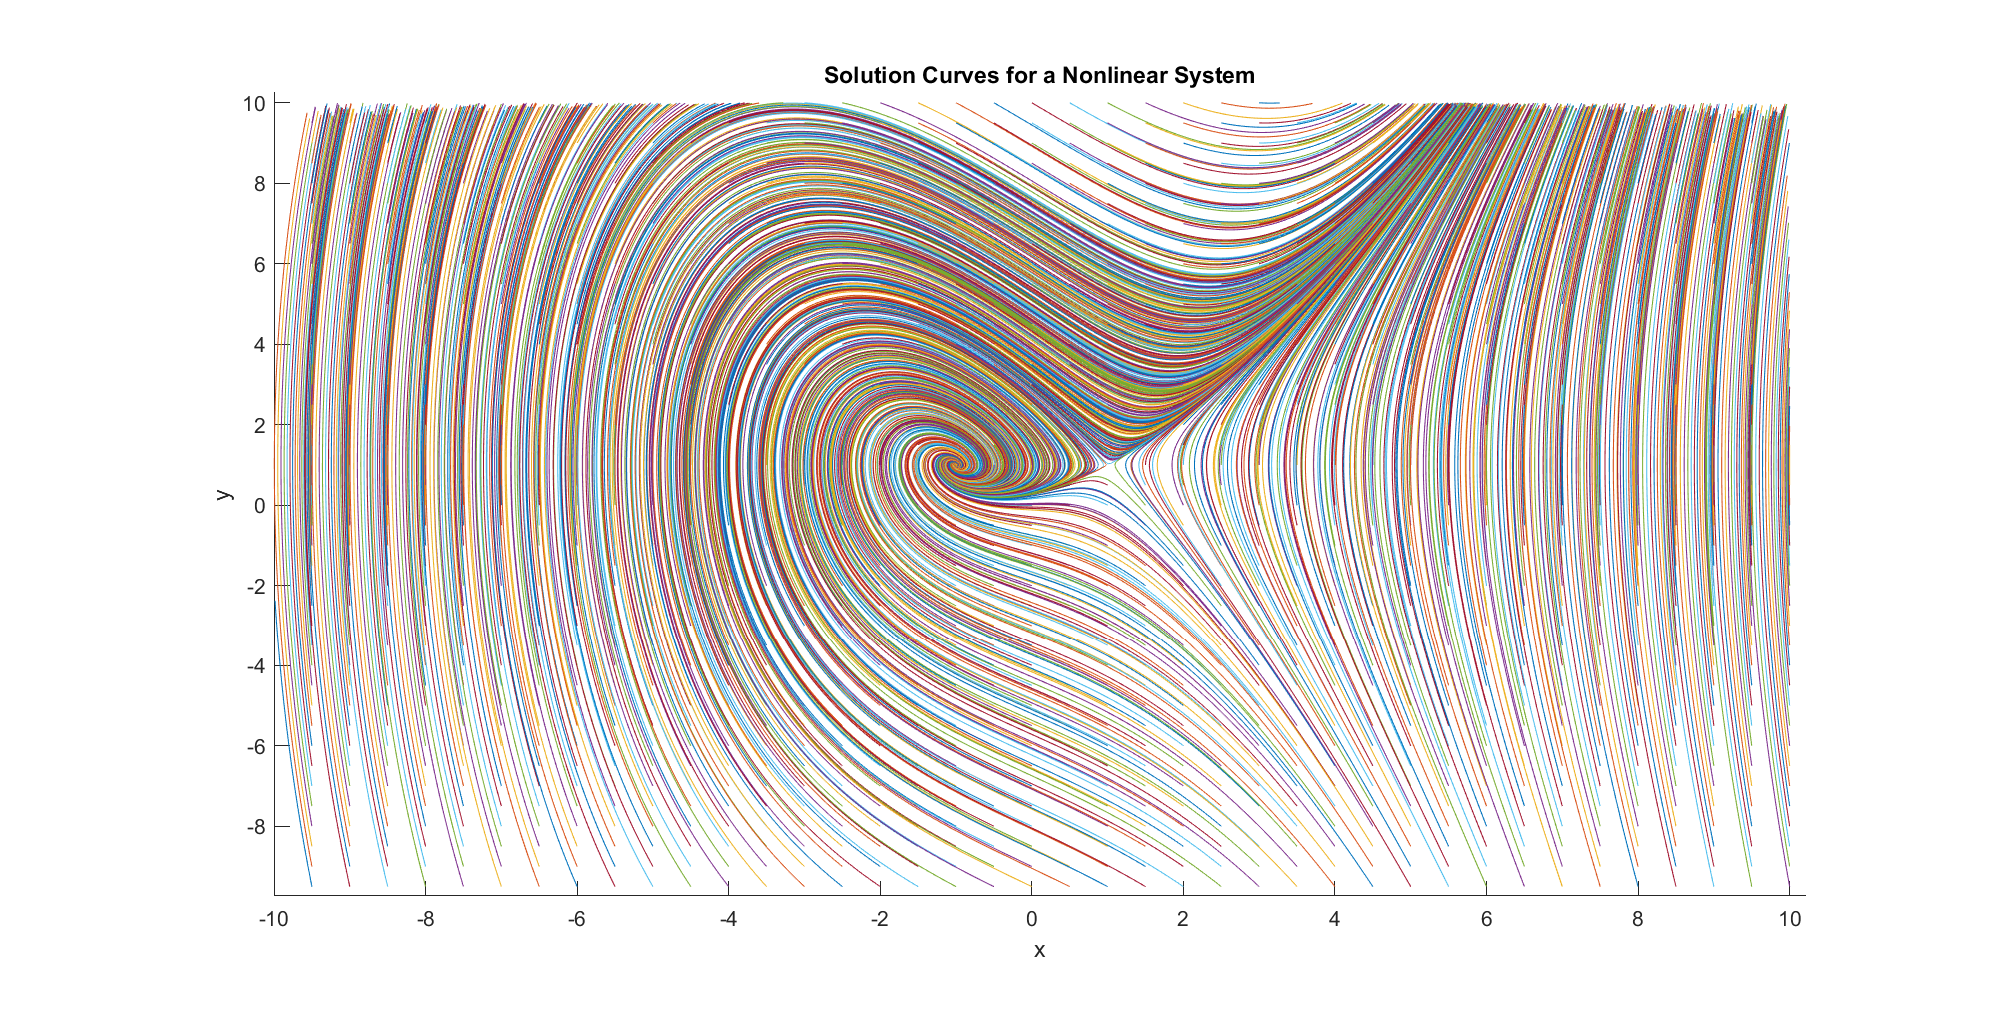
\includegraphics[width=1\linewidth]{NonlinearSystem}
                \end{figure}
            \end{center}
        \end{column}
    \end{columns}

\end{frame}

%------------------------------------------------

\begin{frame}
    \frametitle{The Lorenz System}

    \begin{itemize}
        \item{The Lorenz system is a three-dimensional system of nonlinear differential equations, defined below:}

        \begin{equation}
            \begin{array}{c c l}
                x' & = & \sigma(y - x) \\
                y' & = & \rho x - y - xz \\
                z' & = & xy - \beta z
            \end{array} 
        \end{equation}

        with the restrictions that $\sigma, \rho, \beta > 0$ and $\sigma > \beta + 1$.

        \item{These equations roughly model 2-dimensional fluid convection.}
        % X is the convective overturning
        % Y and Z are horizontal and vertical temperature variation
        % Models a 2D atmosphere with one type of particle
    \end{itemize}
    \begin{figure}
        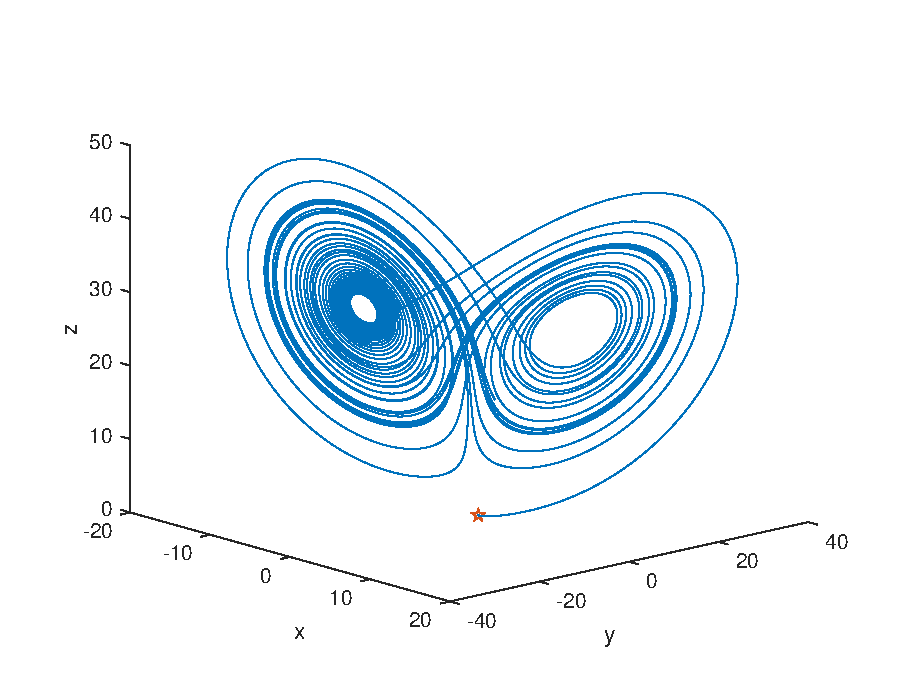
\includegraphics[width=0.4\linewidth]{r28}
    \end{figure}

\end{frame}

%------------------------------------------------

\begin{frame}
    \frametitle{Basic properties of the Lorenz system}

    A few properties are quickly apparent from the Lorenz equations.

    \bigskip

    \begin{itemize}
        \item{The Lorenz equations only have two nonlinearities, but can still exhibit complex, chaotic behavior.}
        \item{The system has symmetry about the z-axis. Therefore, every solution $x(t)$, $y(t)$, $z(t)$ is either symmetric itself, or has a symmetric parter.}
        \item{The system is invariant about the z-axis.}
    \end{itemize}

\end{frame}

%------------------------------------------------

\section{Methods}

% Talk about finite difference methods: Euler, RK4
\begin{frame}
    \frametitle{Methods}
    \framesubtitle{Finite difference methods}
    \begin{itemize}
        \item{Finite difference methods involve approximating the solutions to differential equations by taking small, discrete steps forward from some initial condition.}
        \item{These methods rely on information about a function's derivatives to approximate the original function.}
        \item{For example, Euler's method is defined as $y_{n+1} = y_n + \Delta x \cdot f_n(x,t)$.} % applied to...
        \item{We used numerical simulation in MATLAB, using the 4\textsuperscript{th} order Runge-Kutta method.}
    \end{itemize}
\end{frame}

%------------------------------------------------

\section{Properties}

% derivatives are zero
\begin{frame}
    \frametitle{Fixed Points}

    A \textit{fixed point} of the Lorenz system is a point $(x, y, z)$ such that $x' = y' = z' = 0$. 

    \bigskip

    \begin{itemize}
    \item{If the system reaches one of these states, it will remain there for all time.}
    \item{These fixed points can be shown to be $(0, 0, 0)$ and $\left(\pm\sqrt{\beta(\rho-1)}, \pm\sqrt{\beta(\rho-1)},\rho-1\right)$.}
    \item{We can categorize these fixed points as \textit{stable} and \textit{unstable}, depending on whether trajectories are attracted to or repelled from the fixed point.}
    \end{itemize}

\end{frame}

%------------------------------------------------

\section{Bifurcations}

\begin{frame}
    \frametitle{Bifurcations}
    \begin{itemize}
        \item{As we change the values of parameters $\sigma$, $\rho$, and $\beta$, what happens to the dynamics of the system?}
        \item{We can see from the previous slide that the coordinates of the fixed points are dependent on the system parameters.}
        \item{Changes in number or type of fixed points and limit cycles are called \textit{bifurcations}.}
        \item{We were interested in what happens as the parameter $\rho$ increases. As it increases from 0 to a critical value $\rho^*$, the behavior goes from stable to chaotic.}
    \end{itemize}
\end{frame}

\begin{frame}
    \frametitle{Stable Lorenz Configuration}
    \begin{figure}
        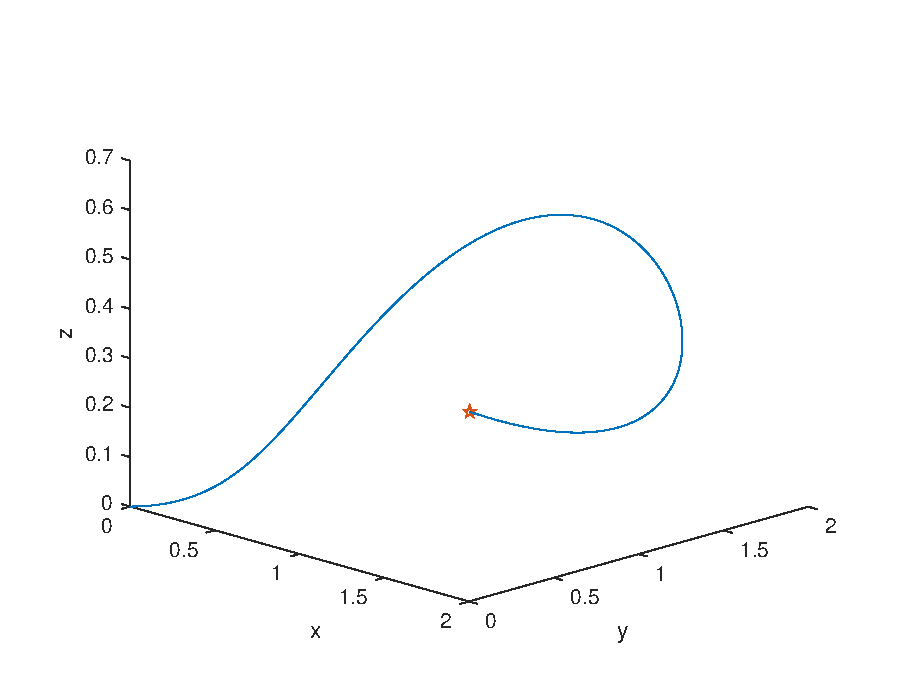
\includegraphics[width=0.7\linewidth]{r05}
        \caption{$\sigma = 10$, $\rho = 0.5$, $\beta = 8/3$}
    \end{figure}
\end{frame}

%------------------------------------------------

\subsection{Bifurcations in Parameter $\rho$}

\begin{frame}
    \frametitle{Bifurcation at $\rho=1$}
    \begin{figure}
        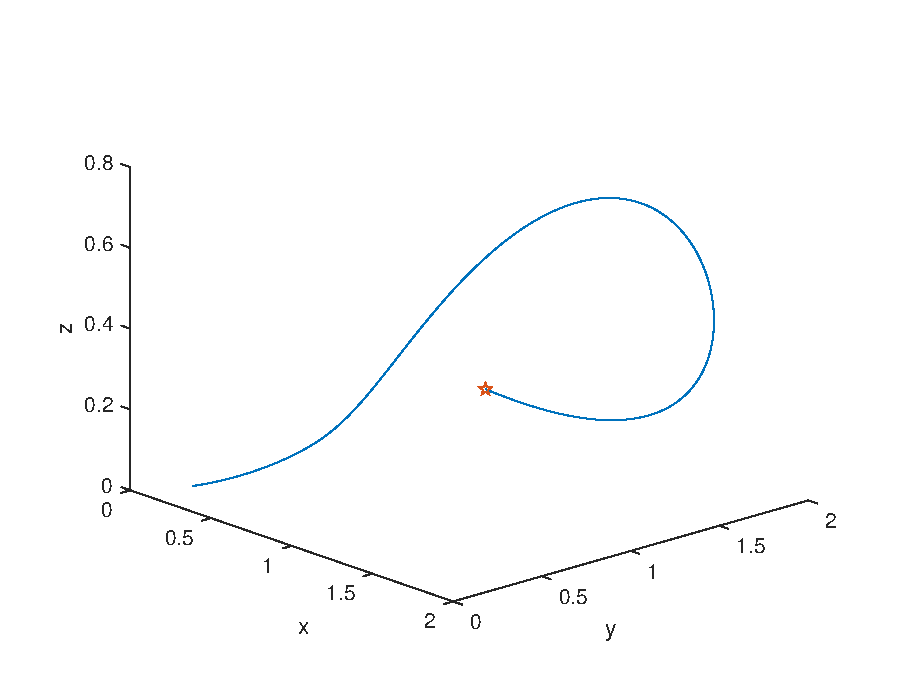
\includegraphics[width=0.7\linewidth]{r1}
        \caption{$\sigma = 10$, $\rho = 1$, $\beta = 8/3$}
    \end{figure}
\end{frame}

%------------------------------------------------

\begin{frame}
    \frametitle{Changing dynamics}
    \begin{figure}
        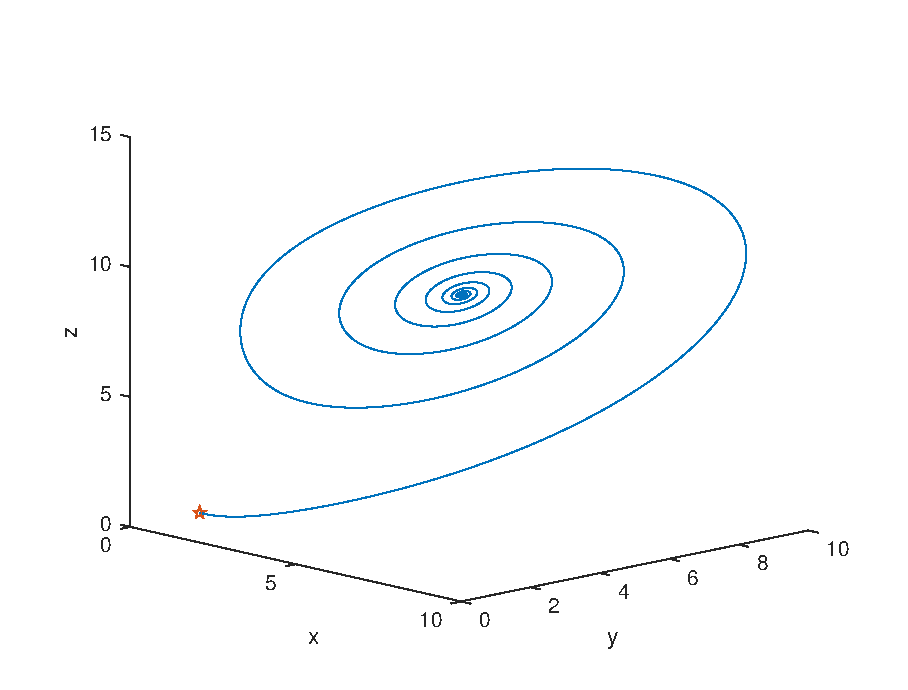
\includegraphics[width=0.7\linewidth]{r10}
        \caption{$\sigma = 10$, $\rho = 10$, $\beta = 8/3$}
    \end{figure}
\end{frame}

%------------------------------------------------

\begin{frame}
    \frametitle{Changing dynamics}
    \begin{figure}
        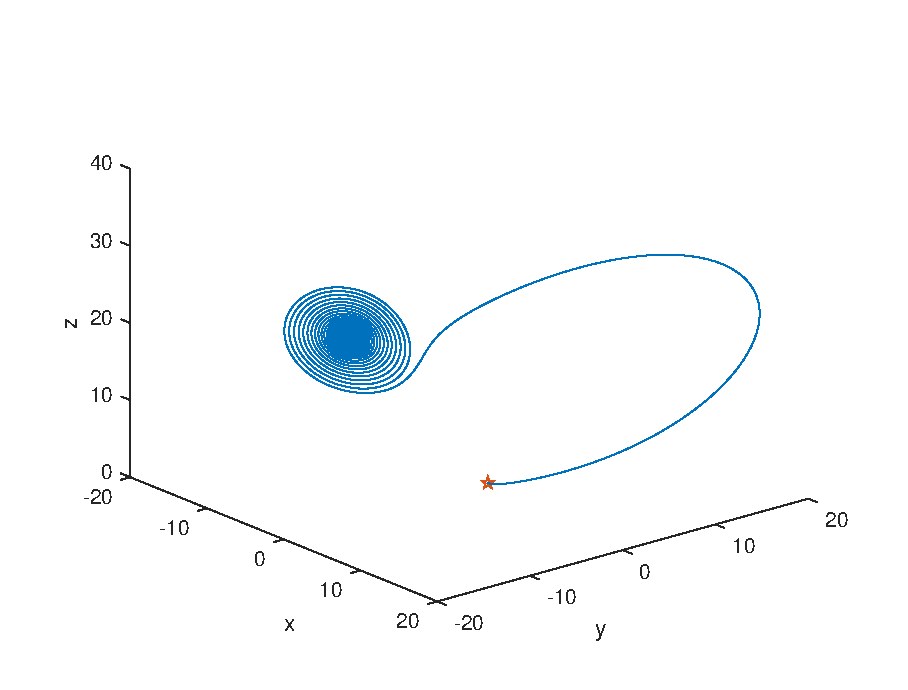
\includegraphics[width=0.7\linewidth]{r20}
        \caption{$\sigma = 10$, $\rho = 20$, $\beta = 8/3$}
    \end{figure}
\end{frame}

%------------------------------------------------

\begin{frame}
    \frametitle{Just under threshold $\rho$}
    \begin{figure}
        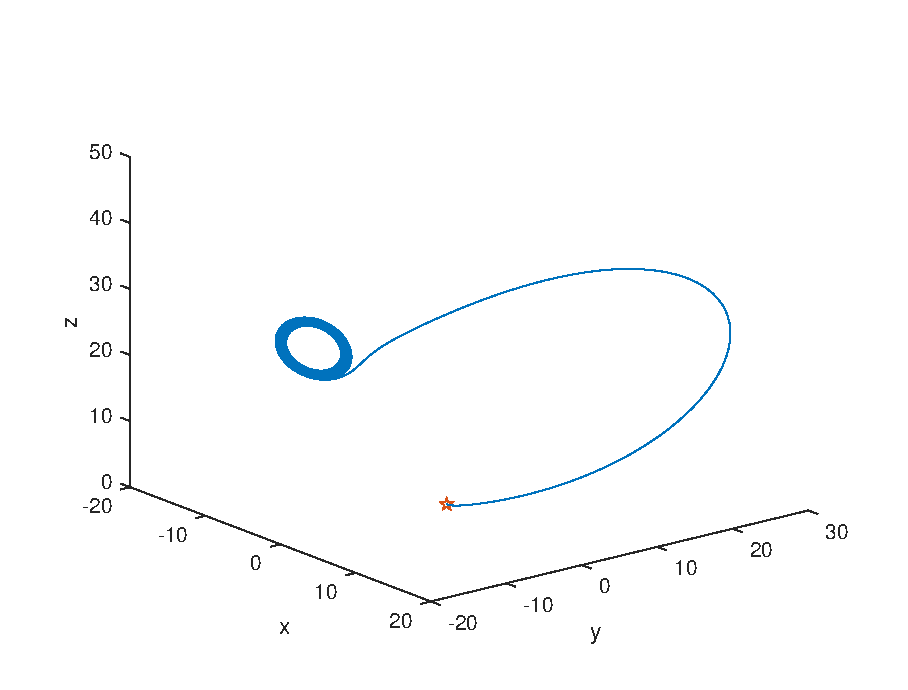
\includegraphics[width=0.7\linewidth]{r24}
        \caption{$\sigma = 10$, $\rho = 24$, $\beta = 8/3$}
    \end{figure}
\end{frame}

%------------------------------------------------

\begin{frame}
    \frametitle{Just over threshold $\rho$}
    \begin{figure}
        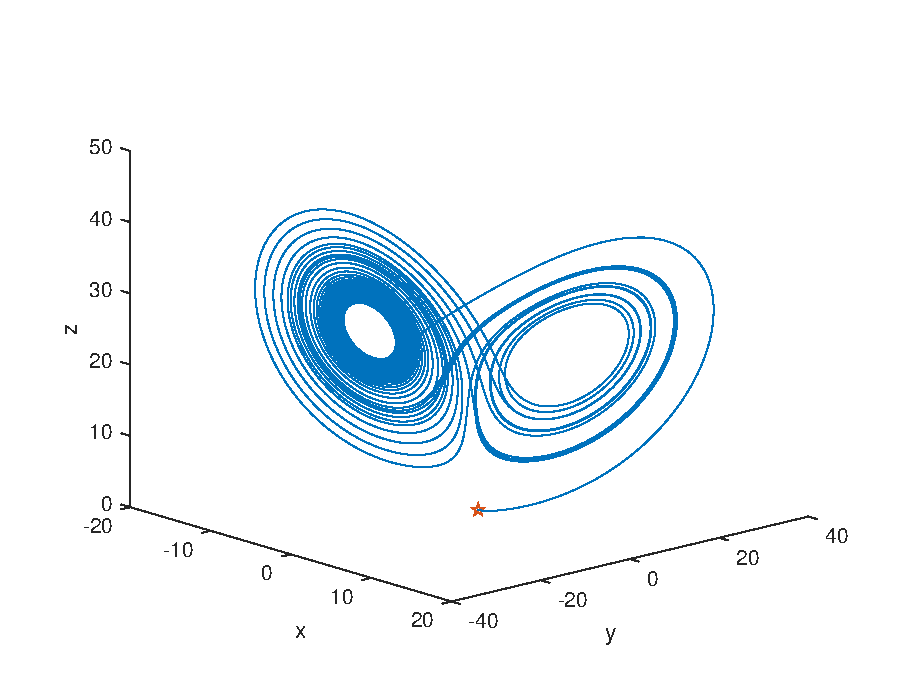
\includegraphics[width=0.7\linewidth]{r25}
        \caption{$\sigma = 10$, $\rho = 25$, $\beta = 8/3$}
    \end{figure}
\end{frame}

%------------------------------------------------

\begin{frame}
    \frametitle{Lorenz's original parameters}
    \begin{figure}
        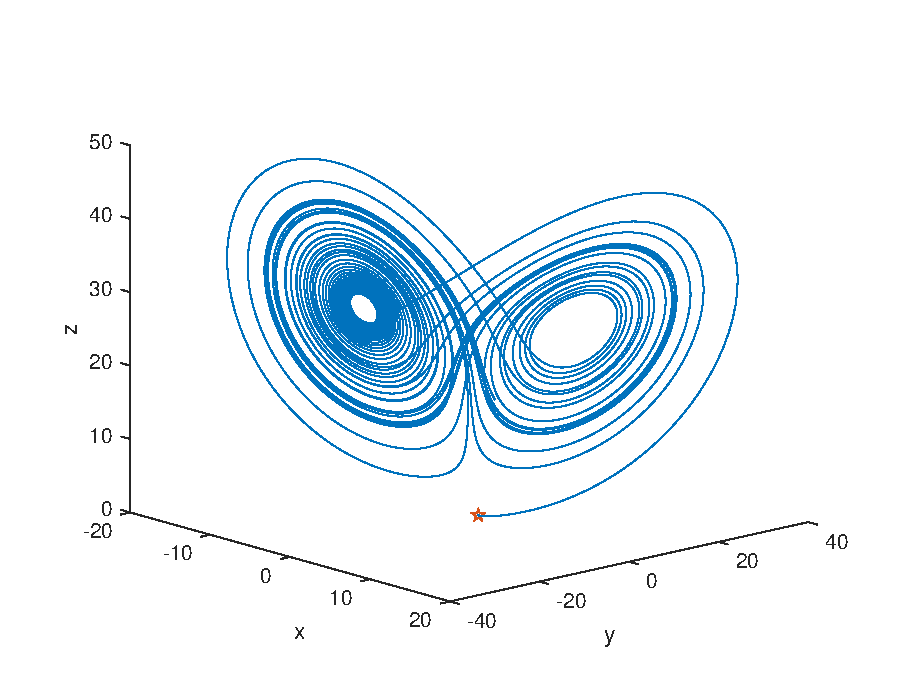
\includegraphics[width=0.7\linewidth]{r28}
        \caption{$\sigma = 10$, $\rho = 28$, $\beta = 8/3$}
    \end{figure}
\end{frame}

%------------------------------------------------

\section{Sensitive Dependence on Initial Conditions}

\begin{frame}
    \frametitle{Sensitive Dependence on Initial Conditions}
    \begin{itemize}
        \item{Two different initial conditions in a chaotic regime of the Lorenz system will always diverge onto unrelated trajectories in finite time, even if they start extremely close.}
        \item{This makes long-term prediction of the system's behavior impossible without direct simulation.}
    \end{itemize}
\end{frame}

%------------------------------------------------

\begin{frame}
    \frametitle{Sensitive Dependence on Initial Conditions}
    \begin{figure}
        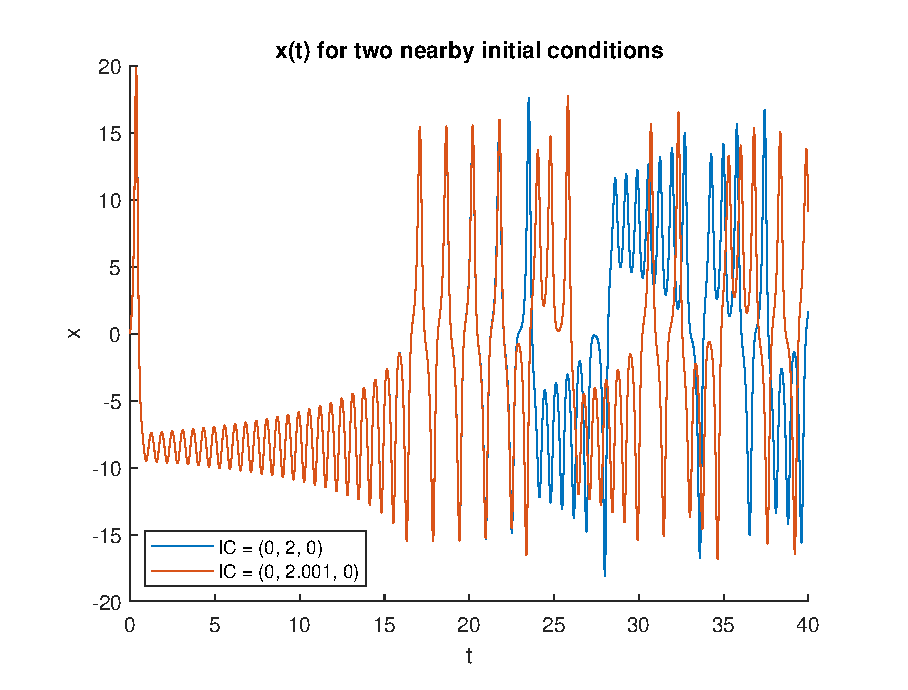
\includegraphics[width=0.8\linewidth]{SDOIC}
    \end{figure}
\end{frame}

%------------------------------------------------

\begin{frame}
    \frametitle{Chaos and the Lorenz System}
    Most definitions of chaos in the context of dynamical systems include the following three parts:

    \bigskip

    \begin{enumerate}
        \item{A deterministic system}
        \item{Aperiodic long-term behavior}
        \item{Sensitive dependence on initial conditions}
    \end{enumerate}

    \bigskip

    The Lorenz system exhibits all three of these properties for certain values of $\sigma$, $\rho$, and $\beta$, so we can characterize its behavior as chaotic.

\end{frame}

%------------------------------------------------

\begin{frame}
    \frametitle{Acknowledgements}
    I want to thank the following people for making this possible:
    \bigskip
    
    \begin{itemize}
        \item{Collin Kofroth}
        \item{The Directed Reading Program committee}
        \item{Everyone here today}
    \end{itemize}
\end{frame}

%------------------------------------------------

\begin{frame}
    \frametitle{References}
    \footnotesize{
    \begin{thebibliography}{99} % Beamer does not support BibTeX so references must be inserted manually as below
        \bibitem{p0} Lorenz (1963)
        \newblock Deterministic Nonperiodic Flow
        \newblock \emph{Journal of the Atmospheric Sciences} 20 (2), 130 -- 141.

        \bibitem{p1} Hirsch, Smale, Devaney (2013)
        \newblock Differential Equations, Dynamical Systems, and an Introduction to Chaos

        \bibitem{p2} Strogatz (1994)
        \newblock Nonlinear Dynamics and Chaos
    \end{thebibliography}
    }
\end{frame}

%------------------------------------------------

\begin{frame}
\Huge{\centerline{The End}}
\end{frame}

%------------------------------------------------

\end{document}